\chapter{Martas Work}


%%%%%%%%%%%%%%%%%%%%%%%%%%%%%%%%%%% MORPHOLOGY %%%%%%%%%%%%%%%%%%%%%%%%%%%%%%%%%%%%%%%%%%%

\section{Morphology}
Morphology is a collection of operations used to analyse and process structures. Although this techniques were commonly used on binary images, nowadays it is possible to apply them also to grayscale images.
The processes related to morphology on binary images are oriented to remove noise produced by thresholding the image as well as define the contours of the objects in order to achieve a proper BLOB analysis.

Mathematical morphology is a neighborhood processing method that applies a \textit{structuring element} (or kernel) to the pixels on the image. The ways that kernel will be structured, how big it will be or the shape that will be used depends on the designer, and the shape and size of the objects to be analysed. The reason for this is that the structured elements are applied by \textit{hitting} or \textit{fitting} operations that will affect the results in different ways.

\subsubsection{Hit and Fit}
Whenever you decide to apply a structured element and \textbf{hit} the pixels, what you are actually doing is to calculate the value of the output pixel by comparing the values of the pixels on the input image and the kernel. The kernel will be first placed on the corner of the image so that it can check if each pixel placed at the same position is also a '1'. If one of the pixels of the area of the kernel is indeed a '1', the pixel in which the kernel is centred will be changed to the value '1' on the output image. Otherwise, the value of the output pixel in that particular position will be '0'.
\begin{figure}[htbp]
\centering
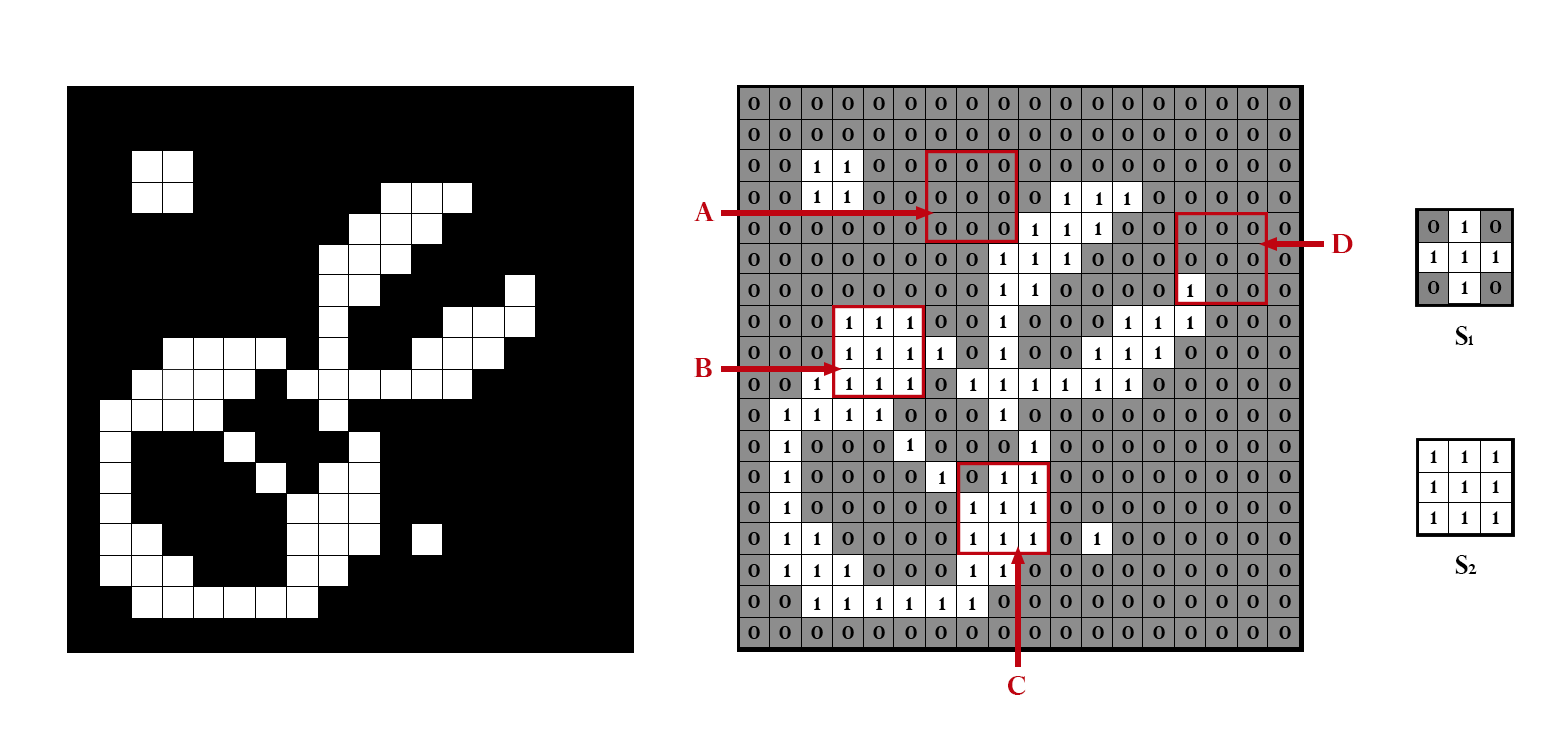
\includegraphics[width=1\textwidth]{Pictures/Theory/FitHitKernels.png}
\caption{Binary image and \textit{Structuring elements}}
\label{fig:FitHit}
\end{figure}

On the contrary, to be able to \textbf{fit} a pixel on the center of the structured element, the pixels' values have to be the same both on the kernel and the input image. If one of the pixels on the input image has a different value to the corresponding '1's of the kernel, the pixel in which the kernel is centred will be a '0' on the output image. On Table \ref{tab:HitFitResults} Figure \ref{fig:FitHit} has been represented with two different types of structuring elements.
\begin{table}[htbp]
\centering
\begin{tabular}{|c|c|c|c|}
\hline
 \:Position\: &SE &\:\:\:Hit\:\:\: &\:\:\:Fit\:\:\: \\\hline
 \hline
 A &$S_{1}$ &No &No\\\hline
 A &$S_{2}$ &No &No\\\hline
 B &$S_{1}$ &Yes &Yes\\\hline
 B &$S_{2}$ &Yes &Yes\\\hline
 C &$S_{1}$ &Yes &Yes\\\hline
 C &$S_{2}$ &Yes &No\\\hline
 D &$S_{1}$ &No &No\\\hline
 D &$S_{2}$ &No &No\\\hline
\end{tabular}
\caption{Results of Hitting and Fitting with two different structuring elements}
\label{tab:HitFitResults}
\end{table}

%%%%%%%%%%%%%%%%%%%%%% SHOULD I TALK A BIT MORE ABOUT THE TABLE? %%%%%%%%%%%%%%%%%%%%%%%%%%%%

\subsection{Dilation}

Dilation is the process of applying Hit to an entire image and refers to the expansion of an object on an image (see Eq. \ref{Dilation1} for a mathematical definition). The result of this method implies also filling small holes and merging objects. As said before, the final effect on these objects will depend on the structured element (how big it is, which shape it has and what values is holding), this can be seen on Figure . 
\begin{equation}
\begin{aligned}
{g(x, y)}={f(x,y)}\oplus{SE}
\label{Dilation1}
	\end{aligned}
\end{equation}
A small structured element applied several times will have the same effect as a big structured element passed once. This can be seen on Eq \ref{Dilation2}, where dilating twice with the element {$SE_{1}$} has the same consequences on the object as dilating one time with {$SE_{2}$}, even though the only difference between those two kernels is that {$SE_{2}$} has a radius twice times bigger than the radius of {$SE_{1}$}.
\begin{equation}
\begin{aligned}
{f(x,y)}\oplus{SE_{2}} \approx ({f(x,y)}\oplus{SE_{1}})\oplus{SE_{1}}
\label{Dilation2}
	\end{aligned}
\end{equation}
\begin{figure}[htbp]
\centering
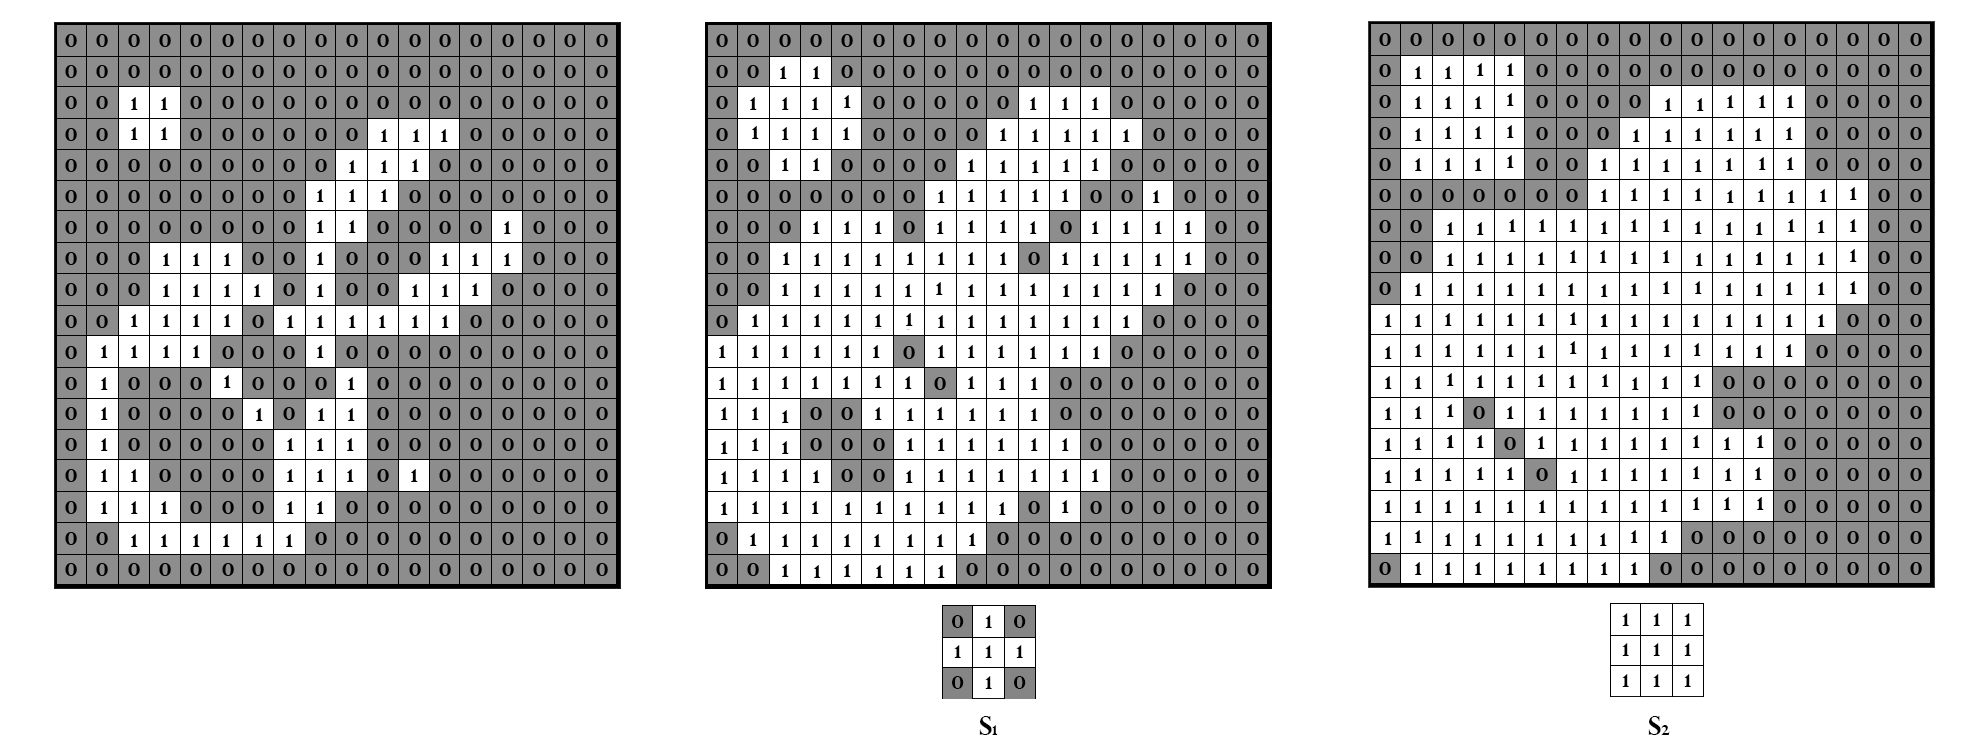
\includegraphics[width=1\textwidth]{Pictures/Theory/Dilation.png}
\caption{Dilation produced by two different structuring elements.}
\label{fig:Dilation}
\end{figure}
%%%%%%%%%%%%%%%%%%%%%%%%% INSERT IMAGES WITH DILATIONS %%%%%%%%%%%%%%%%%%%%%%%%%%%%%%%%%%%%
\subsection{Erosion}
The Erosion is the process of applying Fit to an entire figure and refers to the reduction of the size of an object in an image (the mathematical definition is provided on Eq. \ref{Erosion1}). As the Fit method is applied, small objects will also disappear and larger objects will be break down into smaller ones. As occuring with Dilation, the effects depend on the size, shape and values of the structured element.
\begin{equation}
\begin{aligned}
{g(x, y)}={f(x,y)}\ominus{SE}
\label{Erosion1}
	\end{aligned}
\end{equation}
%%%%%%%%%%%%%%%%%%%%%%%%% INSERT IMAGES WITH EROSIONS %%%%%%%%%%%%%%%%%%%%%%%%%%%%%%%%%%%%
\subsection{Compound Operations}
The term Compound Operations refers to the combination of dilating and eroding objects on an image and can therefore imply the \textit{Union} or \textit{Intersection} of the objects, but also other operations like \textit{Closing}, \textit{Opening} or doing edge detection, also know by \textit{Boundary detection}.
\subsubsection{Opening}
When \textit{eroding} images to erase small noise objects or split parts, it often occurs that the object of interest has decreased its size. The solution to this problem passes by dilating the eroded object. This operation is denoted \textit{Opening} and its mathematical definition is
\begin{equation}
\begin{aligned}
{g(x,y)}={f(x,y)}\circ{SE}=({f(x,y)}\ominus{SE})\oplus{SE}
\label{Opening}
	\end{aligned}
\end{equation}
The effect of Opening can be appreciated on Fig. , where a kernel of ---- is applied to an image. Most of the noise is removed but the object still conserves its original size due to the fact that both structured elements on the Dilation and Erosion have the same size and shape.
\subsubsection{Closing}
Another situation that often occurs when applying these methods comes from \textit{dilating} objects. When the size of the object is increased but it is still important to constrain the measure as well as filling the holes of the objects, a good solution will be to Erode after the Dilation. This is what Closing stands for and it is denoted by the formula \ref{Closing}. As happens with the Opening method, the size and shape must of the kernel be the same in order to obtain the desired result.
On Fig. ---- we can observe the effect of this operations: even though the the holes are filled and the object maintains its original size, the noise of the background is still there. Therefore, it will be necessary to apply either Closing or a BLOB analysis method to delete those small objects.
\begin{equation}
\begin{aligned}
{g(x,y)}={f(x,y)}\bullet{SE}=({f(x,y)}\oplus{SE})\ominus{SE}
\label{Closing}
	\end{aligned}
\end{equation}
It is also important to remember that we can imply the Closing or Opening methods only one time. Most of the holes of the image will be filled but the size of the object will be the original one. If these operations are applied a second time, the size of the final image will be decreased or increased respectively.
%%%%%%%%%%%%%%%%%%%%%%%%%%%%%%%%%%% IMAGE %%%%%%%%%%%%%%%%%%%%%%%%%%%%%%%%%%%%%%%%%%%%%%%%%

\subsubsection{Boundary Detection}
An alternative approach to the edge detection on binary images is the denoted \textit{Boundary Detection}. The performance of this operations is a compound of \textit{erosion} and \textit{subtraction}. Hence the first operation will be eroding the object to get a smaller version of it and then subtract it to the original input image so as to get a final output image with the border of the object. The mathematical definition of these operations is
\begin{equation}
\begin{aligned}
{g(x,y)}={f(x,y)}-({f(x,y)}\ominus{SE})
\label{BoundDetec}
	\end{aligned}
\end{equation}
When the purpose of implementing these operations is to find the edges, it is important to remember to apply first dilation or erosion to remove the noise of the image. The results can be noted on Fig. -----, where the final result is a thin edge of the object.